\chapter{Transport Layer}
The Transport Layer provides logical communication between application processes.
Given an application message, the Transport Layer encapsulates it into one or more packets, called \keyword{segments} (for connection-oriented protocols) or \keyword{datagrams} (for connectionless protocols).

The Transport Layer is fundamentally about process-to-process delivery. 
From the perspective of an application, a process sees communication with another process, even on a different host, as if they were running on the same system. The Transport Layer does not concern itself with the physical routing of packets; it delegates the host-to-host delivery to the underlying Network Layer.

The Transport Layer provides its services through \emph{sockets}, which act as the programming interface between the application and the network. In UNIX systems, sockets are treated like file descriptors: writing into a socket is logically a communication operation.

To achieve process-to-process delivery, the Transport Layer utilizes ports. A \keyword{port} is a 16-bit identifier that uniquely designates a specific receiving endpoint (a socket) on a host. 
An application process relies on one or more sockets to send and receive data, and each socket is bound to a specific port number. When a process transmits data, it pushes the data through its socket. On the receiving end, the host's operating system inspects the destination port number in the incoming packet and directs the data to the corresponding socket, allowing the destination process to retrieve it.

\section{User Datagram Protocol}
The \emph{User Datagram Protocol} (\keyword{UDP}), formalized in RFC 768 \cite{rfc768}, is a minimal, connectionless transport-layer protocol. 
It provides a bare-bones service model, meaning it does not establish a handshake or connection prior to transmitting data, nor does it provide reliability guarantees such as delivery confirmation, strict ordering, or flow control. 
The name \keyword{datagram} is used specifically to emphasize that UDP does not add a significant overhead to IP datagrams \cite{rfc768}. 

\subsection{Datagram Structure}
The UDP datagram is designed for efficiency and minimal latency. 
It consists of a compact 8-byte header followed by the application payload. 
The header contains exactly four fields, each being 16 bits (2 bytes) in length \cite{rfc768}:

\begin{figure}[htbp]
    \centering
    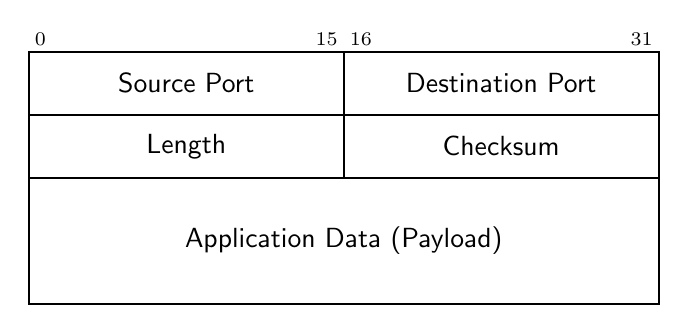
\begin{tikzpicture}[font=\sffamily]
        \def\w{4}
        \def\h{0.8}

        \node[above right, inner sep=2pt, font=\scriptsize] at (0,0) {0};
        \node[above left, inner sep=2pt, font=\scriptsize] at (\w,0) {15};
        \node[above right, inner sep=2pt, font=\scriptsize] at (\w,0) {16};
        \node[above left, inner sep=2pt, font=\scriptsize] at (2*\w,0) {31};

        \draw[thick] (0, 0) rectangle (\w, -\h) node[midway] {Source Port};
        \draw[thick] (\w, 0) rectangle (2*\w, -\h) node[midway] {Destination Port};

        \draw[thick] (0, -\h) rectangle (\w, -2*\h) node[midway] {Length};
        \draw[thick] (\w, -\h) rectangle (2*\w, -2*\h) node[midway] {Checksum};

        \draw[thick] (0, -2*\h) rectangle (2*\w, -4*\h) node[midway] {Application Data (Payload)};
    \end{tikzpicture}
    \caption{Structure of a UDP Datagram}
    \label{fig:udp_datagram}
\end{figure}

\begin{itemize}
    \item \emph{Source Port}: Identifies the port number of the sending process. This field is optional; if the sender does not expect a reply, this field may be set to zero;
    \item \emph{Destination Port}: Identifies the port number of the receiving process, which is critical for \q{routing} the incoming data to the appropriate socket;
    \item \emph{Length}: Specifies the total length of the UDP datagram, which includes both the header and the payload, measured in bytes;
    \item \emph{Checksum}: Used for error detection. The sender computes the checksum over the UDP header, the payload, and a pseudo-header derived from the IP layer. If the receiver calculates a different checksum upon arrival, it assumes the datagram has been corrupted in transit and typically discards it.
\end{itemize}

\subsubsection{Checksum}
In addition to the UDP header and payload, a \emph{pseudo-header} is used in checksum calculation. 
The pseudo-header includes portions of the \emph{IP header} (from the Internet Protocol, IP), even though it is not part of the actual UDP packet. 
It provides additional information about the IP packet being transmitted. The pseudo-header consists of:
\begin{itemize}
    \item Source IP address (\( 4 \) bytes in IPv4, \( 16 \) bytes in IPv6)
    \item Destination IP address (\( 4 \) bytes in IPv4, \( 16 \) bytes in IPv6)
    \item Protocol (\( 1 \) byte) -- always set to \( 17 \) for UDP
    \item UDP length (\( 2 \) bytes) -- the length of the UDP datagram (header + data)
\end{itemize}

\paragraph{Sender Computation}
The sender computes the checksum following a specific sequence of operations \cite{rfc1071}:
\begin{enumerate}
    \item Combine the pseudo-header, UDP header, and UDP payload into a single logical buffer.
    \item Divide the buffer into \( 16 \)-bit words (\( 2 \) bytes each). If the total number of bytes is odd, a padding byte (\texttt{0x00}) is appended to the end.
    \item Sum all the \( 16 \)-bit words together. This arithmetic sum may produce a carry that exceeds \( 16 \) bits.
    \item If the sum is larger than \( 16 \) bits, the overflow is wrapped around; the extra most significant bits are added back to the least significant \( 16 \) bits. This arithmetic is known as one's complement addition.
    \item Complement the final sum (bitwise NOT, flipping all the bits) to produce the final checksum.
    \item The resulting value is placed in the \emph{Checksum} field of the UDP header.
\end{enumerate}

If the calculated checksum evaluates to \( 0 \), it is transmitted as \texttt{0xFFFF} (all ones). A transmitted checksum value of exactly \( 0 \) indicates to the receiver that no checksum was calculated by the sender \cite{rfc768}.

\paragraph{Receiver Computation}
Upon receiving the UDP packet, the receiver validates data integrity by performing the following steps:
\begin{enumerate}
    \item It recomputes the checksum over the pseudo-header, UDP header, and payload using the same one's complement addition.
    \item It adds the newly computed sum to the checksum value received in the UDP header.
    \item If no errors occurred during transmission, this final sum will be all ones (\texttt{0xFFFF}). If the result contains any zeros, the packet is considered corrupted in transit and is typically discarded.
\end{enumerate}

\begin{note}{UDP Checksum in IPv4 vs. IPv6}
In IPv4, the UDP checksum is optional. If a checksum is not utilized, the field is simply set to \( 0 \). Conversely, in IPv6, the UDP checksum is strictly mandatory. This requirement exists because the IPv6 protocol deliberately removed the header checksum at the Network Layer to accelerate packet processing and routing; therefore, error detection must be handled by the Transport Layer.
\end{note}

However, checksums do not guarantee reliable communication: they only ensure the non-corruption of messages, which is just one facet of absolute reliability: we still lack non-lost messages and correct order of messages.

Let's see how to abuild a reliable data transfer (RDT) on top of the unreliable UDP substrate.

\paragraph{Stop-and-Wait}
Let A be the sender and B the receiver.
For A, the simplest way to ensure that B has received a message is to require B to send positive or negative feedback for each message:
\begin{itemize}
    \item B sends a \emph{positive acknowledgement} (\texttt{ACK}) when it has received an intact message from A.
    \item B sends a \emph{negative acknowledgement} (\texttt{NAK}) when it has received a corrupted message from A.
\end{itemize}

This introduces a problem: if B sends a \texttt{NAK} and subsequently receives the same packet again, B cannot immediately know whether this is the resent packet or a delayed duplicate, meaning the \texttt{NAK} itself might have been corrupted.
We can solve this ambiguity by linking messages and their corresponding \texttt{ACK/NAK} with a sequence identifier (ID).
Since the protocol sends only one message at a time, we can implement the ID with a single alternating bit: the first message uses bit \( 0 \), the second uses bit \( 1 \), the third uses \( 0 \), and so on.

Another issue arises if the \texttt{ACK/NAK} does not arrive at all.
A simple yet robust solution is to define a timeout on the sender side: if the \texttt{ACK/NAK} does not arrive within the expected timeout interval, the sender automatically resends the message.
When a timeout triggers, it covers two possible failure scenarios: the \texttt{ACK/NAK} was lost, or the original message was lost.
Since the sender cannot distinguish between the two, it simply resends the message.
When the receiver gets a message, it checks the sequence number. If it is a duplicate, it sends an \texttt{ACK} for the duplicated packet and discards the payload; if it is new, it processes it and sends an \texttt{ACK}. (Modern protocols often drop \texttt{NAK}s entirely in favor of duplicate \texttt{ACK}s).

The behavior of the Stop-and-Wait protocol (often referred to as the alternating-bit protocol) can be formally modeled using Finite State Machines (FSMs).
However, we will first simplify this protocol according to modern practices. In fact, we can drop\texttt{NAK}s entirely in favor of \texttt{ACK}s: when B receives a corrupt datagram or the wrong datagram, it responds by sending an \texttt{ACK} with the flipped bit. So, if B expects to receive a datagram with sequence bit 0, but instead receives the wrong datagram or a corrupted one, B sends an \texttt{ACK} with sequence bit 1.
In this way, the sender has to manage \texttt{ACK}s only: when A is waiting for an \texttt{ACK} with sequence bit 0 but receives instead an \texttt{ACK} with sequence bit 1 or a corrupted datagram, A does nothing and waits possibly for the timeout.
This adaptation simplifies the actual implementation of the protocol.

\begin{figure}[htbp]
\makebox[\textwidth][c]{
    \begin{tikzpicture}[->, >=latex, shorten >=1pt, auto, node distance=5.5cm, semithick, font=\sffamily\footnotesize]
        \node[state, initial] (S0) {Wait for call 0};
        \node[state] (SW0) [right of=S0, xshift=1.5cm] {Wait for ACK 0};
        \node[state] (S1) [below of=SW0, yshift=-1.5cm] {Wait for call 1};
        \node[state] (SW1) [left of=S1, xshift=-1.5cm] {Wait for ACK 1};
        
        \path (S0) edge [bend left] node[above] {\begin{tabular}{@{}c@{}}send(data) \\ \hline send\_dtgm(data, 0) \\ start\_timer\end{tabular}} (SW0)
              (SW0) edge [loop above] node {\begin{tabular}{@{}c@{}}corrupt(rcvd) $\lor$ isACK(rcvd, 1) \\ \hline \emph{do nothing}\end{tabular}} (SW0)
              (SW0) edge [loop right] node {\begin{tabular}{@{}c@{}}timeout \\ \hline resend\_dtgm(data, 0) \\ start\_timer\end{tabular}} (SW0)
                  (SW0) edge [bend left] node[right] {\begin{tabular}{@{}c@{}}$\neg$corrupt(rcvd) $\land$ isACK(rcvd, 0) \\ \hline stop\_timer\end{tabular}} (S1)
              (S1) edge [bend left] node[below] {\begin{tabular}{@{}c@{}}send(data) \\ \hline send\_dtgm(data, 1) \\ start\_timer\end{tabular}} (SW1)
              (SW1) edge [loop below] node {\begin{tabular}{@{}c@{}}corrupt(rcvd) $\lor$ isACK(rcvd, 0) \\ \hline \emph{do nothing}\end{tabular}} (SW1)
              (SW1) edge [loop left] node {\begin{tabular}{@{}c@{}}timeout \\ \hline resend\_dtgm(data, 1) \\ start\_timer\end{tabular}} (SW1)
                  (SW1) edge [bend left] node[left] {\begin{tabular}{@{}c@{}} $\neg$corrupt(rcvd) $\land$ isACK(rcvd, 1) \\ \hline stop\_timer\end{tabular}} (S0);
    \end{tikzpicture}
}
    \caption{Stop-and-Wait Sender FSM. The sender continuously alternates between two main phases: waiting for new data from the application layer, and waiting for an \texttt{ACK} from the receiver. \texttt{dtgm} stands for \emph{datagram}, while \texttt{rcvd} stands for \emph{received}.}
\end{figure}

\begin{figure}[htbp]
    \centering
    \begin{tikzpicture}[->, >=latex, shorten >=1pt, auto, node distance=9cm, semithick, font=\sffamily\footnotesize]
        \node[state, initial] (R0) {Wait for 0};
        \node[state] (R1) [right of=R0] {Wait for 1};
        
        \path (R0) edge [bend left] node[above] {\begin{tabular}{@{}c@{}}$\neg$corrupt(rcvd) $\land$ rcvd.seq = 0 \\ \hline extract(rcvd) \\ deliver(data) \\ sendACK(0)\end{tabular}} (R1)
              (R0) edge [loop above] node {\begin{tabular}{@{}c@{}}corrupt(rcvp) $\lor$ rcvd.seq = 1 \\ \hline sendACK(1)\end{tabular}} (R0)
                  (R1) edge [bend left] node[below] {\begin{tabular}{@{}c@{}}$\neg$corrupt(rcvd) $\land$ rcvd.seq = 1 \\ \hline extract(rcvd) \\ deliver(data) \\ sendACK(1)\end{tabular}} (R0)
              (R1) edge [loop above] node {\begin{tabular}{@{}c@{}}corrupt(rcvp) $\lor$ rcvd.seq = 0 \\ \hline sendACK(0)\end{tabular}} (R1);
    \end{tikzpicture}
    \caption{Stop-and-Wait Receiver FSM. The receiver waits for a specific alternating sequence number (\(0\) or \(1\)). Upon receiving the correct, uncorrupted packet, it delivers the payload and sends an \texttt{ACK}. If it receives a corrupted packet or a duplicate (the incorrect sequence number), it simply discards the payload and resends an \texttt{ACK} for the last successfully received packet to prompt the sender to move forward.}
\end{figure}

Since this communication pattern handles one datagram at a time, and it ensures datagrams are successfully acknowledged and uncorrupted, it inherently preserves the order of messages, establishing a reliable channel.

Stop-and-Wait is functionally simple, but highly inefficient.
It assumes that the time required to create and inject the datagram into the link is much smaller than the time required for the datagram to travel to the receiver and back---represented as the Round Trip Time (\( \text{RTT} \)).
This causes the hosts to sit idle most of the time. To utilize this idle time effectively, we can send several datagrams sequentially before requiring an \texttt{ACK}.
Because we send multiple messages at once, we must pass from sequence bits to sequence numbers.
There are two primary pipelined approaches that improve upon Stop-and-Wait: Go-Back-N and Selective Repeat \cite{kurose2017}.

\paragraph{Go-Back-N (GBN)}
The sender maintains a sliding window representing the allowable range of unacknowledged packets. The window is defined by two primary pointers: \texttt{base}, the sequence number of the oldest\footnote{It is the oldest since it was the first being sent.} unacknowledged datagram; \texttt{next\_seq\_num}, the sequence number of the next datagram to be sent.

The sender can transmit up to \( N \) unacknowledged datagrams. Datagrams within this window are transmitted in order.
GBN uses \emph{cumulative acknowledgements}: an \texttt{ACK} for sequence number \( n \) indicates that all packets up to and including \( n \) have been correctly received.
If a timeout occurs for the packet at the \texttt{base} index, the sender fundamentally assumes failure for the entire unacknowledged window and is forced to resend all unacknowledged packets starting from \texttt{base}.\footnote{This regression in the transmission sequence is exactly why the protocol is named "Go-Back-N".}

The receiver operates very simply: it only keeps track of the next expected sequence number. When it receives the expected datagram, it responds with an \texttt{ACK} for that number and increments its expectation. If it receives an out-of-order datagram, it simply discards it and resends an \texttt{ACK} for the most recently received in-order packet.

\begin{figure}[htbp]
    \centering
    \begin{tikzpicture}[->, >=latex, shorten >=1pt, auto, node distance=7.5cm, semithick, font=\sffamily\footnotesize]
        \node[state, initial, text width=2cm, align=center] (GS) {Wait};
        \path (GS) edge [loop right] node {\begin{tabular}{@{}l@{}}
            send(data)\\
            \hline
            if next\_seq < base + N:\\
            \quad send\_dtgm(data, next\_seq)\\
            \quad if (base == next\_seq) start\_timer\\
            \quad next\_seq++
        \end{tabular}} (GS)
        (GS) edge [loop above] node {\begin{tabular}{@{}l@{}}
            timeout\\
            \hline
            start\_timer\\
            resend\_all(base, next\_seq-1)
        \end{tabular}} (GS)
        (GS) edge [loop below] node {\begin{tabular}{@{}l@{}}
            $\neg$corrupt(rcvd) $\land$ rcvd.seq = base\\
            \hline
            base++\\
            if (base > next\_seq) stop\_timer\\
            else start\_timer
        \end{tabular}} (GS);
    \end{tikzpicture}
    \caption{Go-Back-N Sender FSM. The sender maintains a sliding window of up to \(N\) unacknowledged packets to keep the pipeline full. A single logical timer tracks the oldest unacknowledged packet (the \texttt{base}). Because GBN utilizes cumulative acknowledgements, an \texttt{ACK} shifts the window forward. If the timer expires, the sender assumes all unacknowledged packets in the current window were lost and retransmits them all. The condition \texttt{base > next\_seq} becomes when all datagram have been sent and \texttt{ACK}ed.}
\end{figure}

\begin{figure}[htbp]
    \centering
    \begin{tikzpicture}[->, >=latex, shorten >=1pt, auto, node distance=7cm, semithick, font=\sffamily\footnotesize]
        \node[state, initial, text width=2cm, align=center] (GR) {Wait for\\expected\_seq};
        
        \path (GR) edge [loop right] node {\begin{tabular}{@{}c@{}}
            $\neg$corrupt(rcvd) $\land$ rcvd.seq = expected\_seq\\
            \hline
            extract(rcvd) \\
            deliver(data) \\
            sendACK(expected\_seq)\\
            expected\_seq++
        \end{tabular}} (GR)
        (GR) edge [loop below] node {\begin{tabular}{@{}c@{}}
            corrupt(rcvd) $\lor$ ($\neg$corrupt(rcvd) $\land$ rcvd.seq $\neq$ expected\_seq)\\
            \hline
            discard(rcvd)\\
            sendACK(expected\_seq - 1)
        \end{tabular}} (GR);
    \end{tikzpicture}
    \caption{Go-Back-N Receiver FSM. The receiver enforces strict sequential ordering. It only accepts a packet if its sequence number exactly matches \texttt{expected\_seq}. If any out-of-order packet arrives, it is immediately discarded without buffering, and the receiver re-acknowledges the highest in-order sequence number it has successfully received.}
\end{figure}

While this protocol remains simple on the receiver side, it suffers from notable performance flaws under poor network conditions:
\begin{itemize}
    \item Out-of-order packets are immediately discarded, resulting in wasted network capacity and unnecessary retransmissions.
    \item When a packet is lost, it often signifies network congestion. Blindly dumping a full window of \( N \) packets back into the network exacerbates the congestion rather than alleviating it.
\end{itemize}

\paragraph{Selective Repeat}
To circumvent the inefficiencies of GBN, Selective Repeat (SR) allows the receiver to individually acknowledge correctly received packets. 
The sender uses individual timers for each unacknowledged packet and retransmits \emph{only} those specific datagrams that fail to receive an \texttt{ACK}, rather than the entire window.

To achieve this, the receiver must also maintain a sliding window. 
When the receiver obtains a datagram, it buffers it if the sequence number falls within its current acceptance window, regardless of whether it is out of order. It sends an individual \texttt{ACK} for that specific packet. If the received packet matches the window's base, the receiver delivers it (along with any previously buffered consecutive packets) to the application layer and shifts the window forward.
When a corrupted datagram arrives to the receiver, it is discarded and no \texttt{ACK} is produced as responding with an \texttt{ACK} would break the described protocol.

\begin{figure}[htbp]
    \centering
    \begin{tikzpicture}[->, >=latex, shorten >=1pt, auto, node distance=7cm, semithick, font=\sffamily\footnotesize]
        \node[state, initial, text width=2cm, align=center] (SRR) {Wait};
        
        \path (SRR) edge [loop right] node {\begin{tabular}{@{}l@{}}
            $\neg$corrupted(rcvd) $\land$ rcvd.seq = $\in$ [base, base + $n$ - 1]\\
            \hline
            sendACK(rcvd.seq)\\
            buffer(rcvd)\\
            if (rcvd.seq == base):\\
            \quad deliver in-order buffered datagrams\\
            \quad base++
        \end{tabular}} (SRR)
        (SRR) edge [loop below] node {\begin{tabular}{@{}l@{}}
            $\neg$corrupted(rcvd) $\land$ rcvd.seq $\not\in$ [base, base + $n$ - 1]\\
            \emph{(Sender's ACK was lost/delayed)}\\
            \hline
            sendACK(rcvd.seq)
        \end{tabular}} (SRR)
        (SRR) edge [loop above] node {\begin{tabular}{@{}l@{}}
            corrupted(rcvd)\\
            \hline
            discard(rcvd)
        \end{tabular}} (SRR);
    \end{tikzpicture}
    \caption{Selective Repeat Receiver FSM. Unlike GBN, the receiver buffers out-of-order packets that fall within its valid acceptance window (\texttt{base} to \texttt{base + N - 1}) and acknowledges them individually. Once the packet corresponding to \texttt{base} arrives, the window shifts forward, and all consecutive buffered packets are delivered to the application layer in one step.}
\end{figure}

\section{Transmission Control Protocol}
The \emph{Transmission Control Protocol} (\keyword{TCP}), formally specified in RFC 793 \cite{rfc793}, is the cornerstone of reliable transport in the Internet architecture. 
Unlike UDP, TCP is intensely connection-oriented, requiring a formal handshake prior to exchanging data. It ensures absolute reliability by recovering from data loss, duplication, and out-of-order delivery. Furthermore, TCP is acutely congestion and flow aware, dynamically adapting its transmission rate to protect both the receiving host and the core network infrastructure from being overwhelmed.

While UDP is suitable for broadcast or multicast communications where loose reliability is acceptable, TCP provides a \emph{full-duplex, point-to-point} connection.
Rather than transmitting independent, isolated datagrams, TCP treats the application data as a continuous \keyword{data stream}. The protocol divides this stream into smaller, manageable chunks called \keyword{segments}. These segments do not inherently preserve application-level message boundaries; they are merely contiguous bytes sliced from the data stream.

To manage potential delays across the application, operating system, and network, TCP communication relies heavily on \emph{buffers}. Both ends of a connection maintain send and receive buffers to temporarily store the stream data until it can be reliably transmitted or consumed by the application layer.

Since the underlying Link Layer imposes a \emph{Maximum Transmission Unit} (\keyword{MTU}), the \emph{Maximum Segment Size} (\keyword{MSS}) -- which defines the maximum amount of application data a single TCP segment can carry -- is constrained by the required headers:
\[
\text{MSS} = \text{MTU} - (\text{headers}_{\text{IP}} + \text{headers}_{\text{TCP}})
\]

\subsection{Segment}
The TCP header is generally \( 20 \) bytes long, though optional fields can extend its length up to \( 60 \) bytes. This deterministic header structure wraps the variable-length application data slice. To understand how TCP guarantees reliability, flow control, and connection state management, it is necessary to examine every single bit of its structure \cite{rfc9293}.

\begin{figure}[htbp]
    \centering
    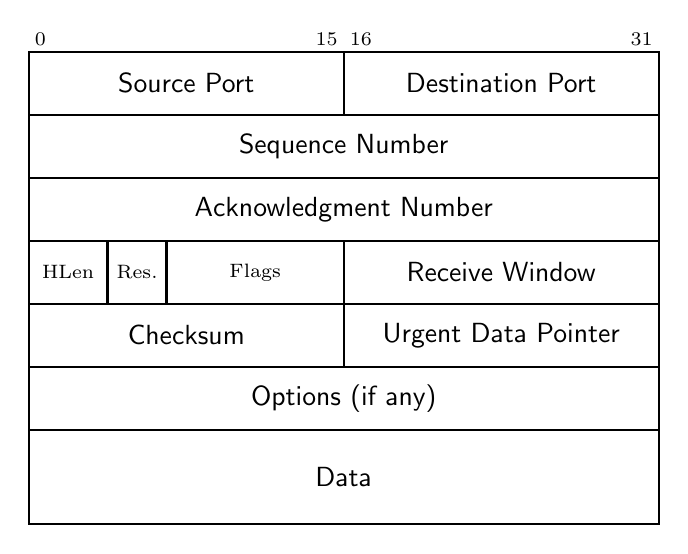
\begin{tikzpicture}[font=\sffamily]
        \def\w{4}
        \def\h{0.8}

        \node[above right, inner sep=2pt, font=\scriptsize] at (0,0) {0};
        \node[above left, inner sep=2pt, font=\scriptsize] at (\w,0) {15};
        \node[above right, inner sep=2pt, font=\scriptsize] at (\w,0) {16};
        \node[above left, inner sep=2pt, font=\scriptsize] at (2*\w,0) {31};

        % Row 1: Ports (16 bits + 16 bits)
        \draw[thick] (0, 0) rectangle (\w, -\h) node[midway] {Source Port};
        \draw[thick] (\w, 0) rectangle (2*\w, -\h) node[midway] {Destination Port};

        % Row 2: Sequence Number (32 bits)
        \draw[thick] (0, -\h) rectangle (2*\w, -2*\h) node[midway] {Sequence Number};

        % Row 3: Acknowledgment Number (32 bits)
        \draw[thick] (0, -2*\h) rectangle (2*\w, -3*\h) node[midway] {Acknowledgment Number};

        % Row 4: HLen (4), Res (3), Flags (9), Window (16)
        % Using precise absolute widths assuming 2*\w = 8. 
        % 32 bits = 8 units. 1 bit = 0.25 units.
        \draw[thick] (0, -3*\h) rectangle (1, -4*\h) node[midway, align=center, font=\scriptsize] {HLen};
        \draw[thick] (1, -3*\h) rectangle (1.75, -4*\h) node[midway, font=\scriptsize] {Res.};
        \draw[thick] (1.75, -3*\h) rectangle (4, -4*\h) node[midway, font=\scriptsize] {Flags};
        \draw[thick] (4, -3*\h) rectangle (8, -4*\h) node[midway] {Receive Window};

        % Row 5: Checksum (16), Urgent Pointer (16)
        \draw[thick] (0, -4*\h) rectangle (\w, -5*\h) node[midway] {Checksum};
        \draw[thick] (\w, -4*\h) rectangle (2*\w, -5*\h) node[midway] {Urgent Data Pointer};

        % Row 6: Options
        \draw[thick] (0, -5*\h) rectangle (2*\w, -6*\h) node[midway] {Options (if any)};
        
        % Data
        \draw[thick] (0, -6*\h) rectangle (2*\w, -7.5*\h) node[midway] {Data};
    \end{tikzpicture}
    \caption{Precise Structure of a TCP Segment}
    \label{fig:tcp_segment}
\end{figure}

The core components of the header include every aspect necessary for the complex state machine of a TCP connection:

\begin{itemize}
    \item \emph{Source and Destination Port Numbers} (\( 16 \) bits each): Port numbers allow to route the segment to the correct application sockets.
    \item \emph{Sequence Number} (\( 32 \) bits): Identifies the position of the data in the sender's byte stream. If the \texttt{SYN} flag is present, this field contains the randomly generated Initial Sequence Number (\keyword{ISN}), and the first data byte is \(\text{ISN} + 1\). Otherwise, it denotes the accumulated byte offset of the first data byte in this segment.
    \item \emph{Acknowledgment Number} (\( 32 \) bits): If the \texttt{ACK} flag is set, this field contains the sequence number of the \emph{next} byte the receiver expects to receive. It acts as a cumulative acknowledgment of all bytes received prior to this number.
    \item \emph{Header Length / Data Offset} (\( 4 \) bits): Specifies the size of the TCP header in \( 32 \)-bit words. Since the minimum header is \( 20 \) bytes, the minimum value is \( 5 \). Its maximum value is \( 15 \), capping the TCP header at \( 60 \) bytes and leaving up to \( 40 \) bytes for Options.
    \item \emph{Reserved} (\( 3 \) bits): Reserved for future use and must be set to zero. (Originally \( 6 \) bits in RFC 793, but later reduced as new flags were introduced).
    \item \emph{Control Flags} (\( 9 \) bits): These bits govern the state of the connection and congestion control mechanics. In exact order from left to right:
    \begin{itemize}
        \item \texttt{NS} (Nonce Sum, \( 1 \) bit): An experimental flag used to protect against accidental or malicious concealment of packets from the sender \cite{rfc3540}.
        \item \texttt{CWR} (Congestion Window Reduced, \( 1 \) bit): Set by the sender to indicate that it received a segment with the \texttt{ECE} flag set and responded by reducing its congestion window \cite{rfc3168}.
        \item \texttt{ECE} (ECN-Echo, \( 1 \) bit): Explicit Congestion Notification Echo. Depending on the \texttt{SYN} flag, it indicates either that the TCP peer is ECN-capable or that network congestion was encountered during transmission \cite{rfc3168}.
        \item \texttt{URG} (Urgent, \( 1 \) bit): Indicates that the Urgent Data Pointer field is significant and contains prioritized data that the application should process immediately.
        \item \texttt{ACK} (Acknowledgment, \( 1 \) bit): Indicates that the Acknowledgment Number field is valid. All segments after the initial \texttt{SYN} packet must have this flag set.
        \item \texttt{PSH} (Push, \( 1 \) bit): Instructs the receiving host to immediately push all buffered data to the receiving application without waiting for the buffer to fill.
        \item \texttt{RST} (Reset, \( 1 \) bit): Immediately aborts the connection, usually in response to an unrecoverable error or an invalid segment.
        \item \texttt{SYN} (Synchronize, \( 1 \) bit): Used exclusively during the three-way handshake to synchronize sequence numbers and initiate a connection.
        \item \texttt{FIN} (Finish, \( 1 \) bit): Indicates that the sender has no more data to transmit, initiating a graceful connection teardown.
    \end{itemize}
    \item \emph{Receive Window} (\( 16 \) bits): Communicates the receiver's available buffer space (in bytes), strictly enforcing \keyword{flow control} so the sender does not overwhelm the receiver's capacity.
    \item \emph{Checksum} (\( 16 \) bits): Validates the integrity of the header, the data payload, and a pseudo-header containing the source and destination IP addresses, ensuring that corrupted segments are discarded.
    \item \emph{Urgent Data Pointer} (\( 16 \) bits): If the \texttt{URG} flag is set, this field holds a positive offset added to the Sequence Number, indicating the sequence number of the last byte in the sequence of urgent data.
    \item \emph{Options} (Variable length): Accommodates advanced features such as the Maximum Segment Size (MSS) negotiation during the handshake, Window Scaling (to exceed the \( 16 \)-bit window limit), Timestamps (for precise RTT calculation), and Selective Acknowledgments (SACK) \cite{rfc9293}.
\end{itemize}

\subsection{Segmentation}
Because TCP treats data as an unstructured stream, the \keyword{Sequence Number} assigned to a segment is not a packet index (e.g., segment 1, segment 2). Rather, it represents the byte-stream position of the \emph{first byte} of the segment's payload within the overall application message. The very first sequence number utilized for a connection is a randomly generated Initial Sequence Number (\keyword{ISN}).

Conversely, the \keyword{Acknowledgment Number} (often abbreviated as ACK) denotes the byte-stream number of the \emph{next byte} the receiver expects to consume. For instance, if an incoming segment contains an ACK number of 100, the sender is formally communicating that it has successfully received contiguous bytes up through byte 99 of the incoming data stream, and is now waiting for byte 100.

\begin{example}{Segmentation in Practice}
Consider an application generating a \( 1000 \)-byte message, and a connection governed by an MSS of \( 100 \) bytes. TCP will segment this message into \( 10 \) individual packets, each carrying a \( 100 \)-byte payload. 
If the sender's ISN is \( 0 \), the first segment's sequence number is \( 0 \). The second segment's sequence number will be \( 100 \), the third will be \( 200 \), and so forth.
\end{example}

Because TCP connections are full-duplex, sequence and acknowledgment numbers work concurrently. Every transmitted segment (except initial handshakes) carries both a Sequence Number referencing the outbound data stream, and an Acknowledgment Number referencing the inbound data stream, with the \texttt{ACK} flag explicitly set.

\subsection{Retransmission}
The foundational reliability mechanism of pipelined TCP is retransmission driven by timeouts. If a segment's associated \texttt{ACK} is not received before a designated timer expires, TCP assumes the segment was lost and retransmits it.

Estimating this timeout interval is highly critical to overall performance:
\begin{itemize}
    \item If the timeout is prematurely short, TCP will trigger unnecessary retransmissions, injecting redundant traffic and artificially exacerbating network congestion.
    \item If the timeout is excessively long, the protocol reacts sluggishly to genuine packet loss, significantly degrading application throughput.
\end{itemize}

The timeout interval must obviously exceed the Round Trip Time (\keyword{RTT}). Because network latency dynamically fluctuates, TCP continually estimates the RTT by measuring the time elapsed between sending a segment and receiving its ACK (an \emph{RTT sample}). 
To smooth out transient fluctuations, TCP maintains an Exponentially Weighted Moving Average for the estimated RTT:
\[
\text{EstimatedRTT}_{t} = (1 - \alpha) \cdot \text{EstimatedRTT}_{t-1} + \alpha \cdot \text{SampleRTT}
\]
Typically, \( \alpha = 1/8 \), affording heavy weight to historical estimations and protecting against sudden, short-lived spikes.

However, recognizing that network delays can exhibit severe variance, TCP also computes an RTT deviation metric to capture the margin of error in its estimation:
\[
\text{DevRTT}_{t} = (1 - \beta) \cdot \text{DevRTT}_{t-1} + \beta \cdot |\text{SampleRTT}_{t} - \text{EstimatedRTT}_{t}|
\]
Typically, \( \beta = 1/4 \).

Ultimately, TCP defines a highly robust timeout interval by combining the estimated RTT with a safety margin based on the calculated deviation \cite{rfc6298}:
\[
\text{TimeoutInterval}_{t} = \text{EstimatedRTT}_{t} + 4 \cdot \text{DevRTT}_{t}
\]
While the initial default timeout is often provisioned at 1 second, this dynamic formula ensures the timer quickly adapts to the prevailing network conditions.

\subsubsection{Fast Retransmit}
Relying solely on timeouts can be slow, especially when long timers are in effect. To accelerate recovery, TCP utilizes \emph{Fast Retransmit} \cite{rfc5681}. 
Because a receiver generates a duplicate ACK every time it receives an out-of-order segment (requesting the missing segment again), the sender can use these duplicate ACKs as a heuristic for packet loss. 
If a sender receives three duplicate ACKs (i.e., four ACKs in total acknowledging the same sequence number), it assumes the packet immediately following the acknowledged byte was lost in the network. The sender will retransmit that segment immediately, without waiting for the timeout interval to expire.

\subsection{Connection Management}
Before transmitting any application data, the TCP sender and receiver must formally establish a connection to synchronize their ISNs and allocate necessary operating system resources (buffers and variables).
Reaching a consensus across an unreliable network is a fundamentally difficult problem, famously modeled as the \emph{Two-Army Problem} \cite{tanenbaum2011}.

\begin{figure}[htbp]
    \centering
    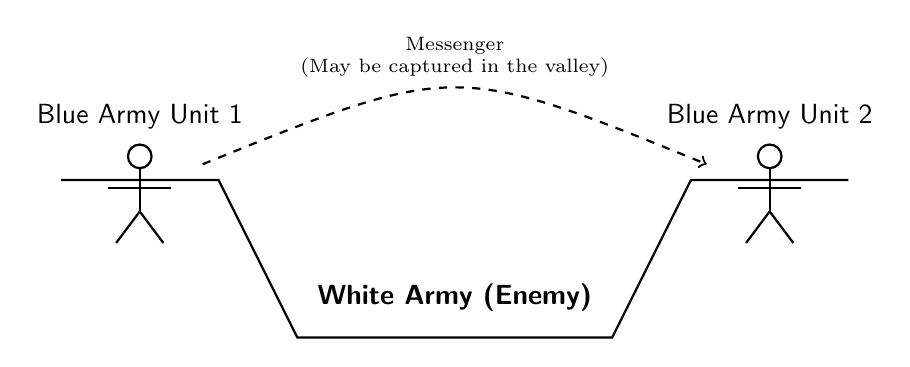
\begin{tikzpicture}[font=\sffamily]
        % Terrain
        \draw[thick] (0,2) -- (2,2) -- (3,0) -- (7,0) -- (8,2) -- (10,2);
        
        % Blue Army 1
        \node at (1,2.8) {Blue Army Unit 1};
        \draw[thick] (1,2.3) circle (0.15); 
        \draw[thick] (1,2.15) -- (1,1.6); 
        \draw[thick] (0.6,1.9) -- (1.4,1.9); 
        \draw[thick] (1,1.6) -- (0.7,1.2); 
        \draw[thick] (1,1.6) -- (1.3,1.2);
        
        % Blue Army 2
        \node at (9,2.8) {Blue Army Unit 2};
        \draw[thick] (9,2.3) circle (0.15); 
        \draw[thick] (9,2.15) -- (9,1.6); 
        \draw[thick] (8.6,1.9) -- (9.4,1.9); 
        \draw[thick] (9,1.6) -- (8.7,1.2); 
        \draw[thick] (9,1.6) -- (9.3,1.2);
        
        % White Army (Valley)
        \node at (5,0.5) {\textbf{White Army (Enemy)}};
        
        % Messenger path
        \draw[dashed, ->, thick] (1.8,2.2) .. controls (5,3.5) .. (8.2,2.2) node[midway, above, align=center, font=\scriptsize] {Messenger\\(May be captured in the valley)};
    \end{tikzpicture}
    \caption{The Two-Army Problem. The blue army can only defeat the white army if both units attack simultaneously. However, they must coordinate by sending messengers through the dangerous valley. Unit 1 sends an attack time, but cannot attack until Unit 2 confirms. Unit 2 confirms, but cannot attack until Unit 1 confirms it received the confirmation. This infinite requirement for acknowledgments proves that reaching absolute certainty over an unreliable channel is impossible.}
    \label{fig:two_army}
\end{figure}

The Two-Army Problem proves that no protocol can guarantee 100\% mutual agreement if messages can be lost. However, while absolute mathematical certainty is impossible, TCP employs a \keyword{three-way handshake} which is practically adequate for establishing reliable connections over the Internet.

\paragraph{Connection Establishment}
The three-way handshake proceeds as follows:
\begin{enumerate}
    \item \texttt{SYN}: The client initiates the connection by sending a TCP segment with the \texttt{SYN} flag set, containing a randomized Initial Sequence Number (ISN) for the client-to-server stream.
    \item \texttt{SYN-ACK}: The server allocates buffers and state variables for the connection. It responds with a segment that has both the \texttt{SYN} and \texttt{ACK} flags set, acknowledging the client's ISN and providing its own randomized ISN for the server-to-client stream.
    \item \texttt{ACK}: The client allocates its own buffers and state variables. It acknowledges the server's ISN by sending a final segment with the \texttt{ACK} flag set. (This third segment may also carry the first bytes of application data).
\end{enumerate}

\begin{note}{SYN-Flood Attacks}
During the handshake, a server must allocate resources upon receiving a SYN segment. Malicious actors exploit this by initiating a \emph{SYN-flood attack}, dispatching vast numbers of SYN requests without ever completing the final ACK \cite{rfc4987}. To mitigate this, modern servers employ strict timeouts for half-open connections and utilize techniques like SYN cookies to defer resource allocation until the handshake is complete.
\end{note}

\paragraph{Connection Release (Teardown)}
When an application is ready to close the connection, TCP uses a graceful teardown process to ensure no data is truncated:
\begin{enumerate}
    \item \texttt{FIN}: The client sends a segment with the \texttt{FIN} flag set, indicating it has no more data to send.
    \item \texttt{FIN-ACK}: The server acknowledges the request with an \texttt{ACK}. At this stage, the server can still transmit remaining data. Once finished, the server sends its own \texttt{FIN} segment. (Often, the server's \texttt{FIN} and \texttt{ACK} are combined into a single segment).
    \item \texttt{ACK}: The client receives the server's \texttt{FIN} and responds with a final \texttt{ACK}. The client then enters a timed wait state to ensure the final acknowledgment wasn't lost before fully deallocating local resources.
\end{enumerate}

\subsection{Congestion and Flow Control}
In modern networks, packet loss is rarely caused by physical line noise; it is predominantly the result of router buffers overflowing during traffic spikes. Overloading the network triggers timeouts, which cause retransmissions, dynamically injecting even more traffic into an already saturated system. 
TCP implements two distinct mechanisms to regulate traffic: \emph{Flow Control} (preventing the sender from overwhelming the specific receiving host) and \emph{Congestion Control} (preventing the sender from overwhelming the intermediate network infrastructure).

\subsubsection{Flow Control}
Flow control acts as a direct speed-matching service between the sender and the receiver, ensuring that the sender does not transmit data faster than the receiving application can process it. 

While implemented as dynamic linked lists of packet structures within modern operating system kernels, the TCP receive buffer is logically abstracted in protocol design as a contiguous, circular array of bytes with a maximum capacity of \texttt{RcvBuffer}. As data flows in from the network and is subsequently read by the application, the logical pointers tracking the data continuously wrap around this circular space \cite{kurose2017}.

To prevent buffer overflow, the receiver continuously calculates its available buffer space and explicitly communicates this value to the sender. This advertised free space is termed the \keyword{receive window} (\texttt{rwnd}).

To understand how this available capacity is computed, we must observe the two primary sequence variables maintained by the receiver's TCP stack:
\begin{itemize}
    \item \texttt{LastByteRead}: The sequence number of the last byte the application layer successfully consumed from the buffer.
    \item \texttt{LastByteRcvd}: The sequence number of the last byte that arrived from the network and was successfully buffered.
\end{itemize}

\begin{figure}[htbp]
    \centering
    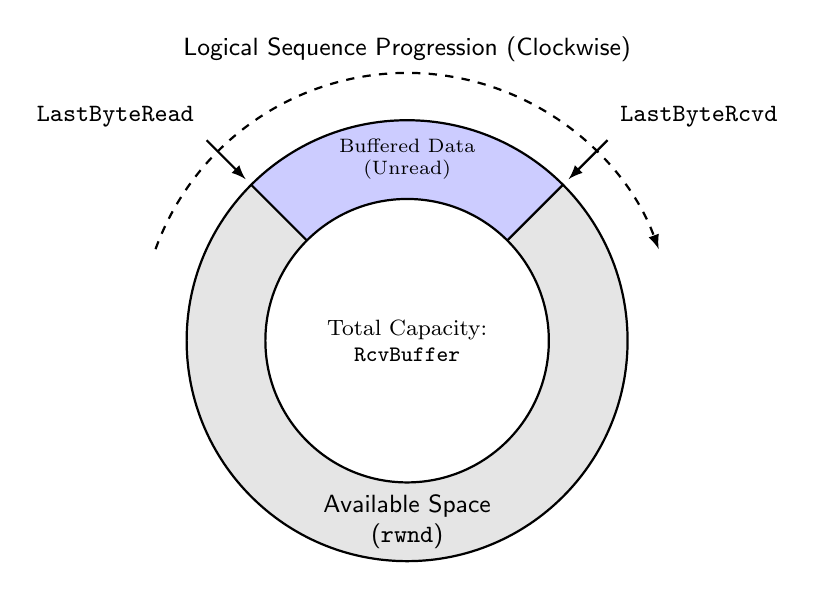
\begin{tikzpicture}[font=\sffamily\small]
        \def\R{2.8}
        \def\r{1.8}
        
        % Fill buffered data (Clockwise from 135 to 45)
        \fill[blue!20] (135:\R) arc (135:45:\R) -- (45:\r) arc (45:135:\r) -- cycle;
        
        % Fill available space (Clockwise from 45 to -225, wrapping around)
        \fill[gray!20] (45:\R) arc (45:-225:\R) -- (-225:\r) arc (-225:45:\r) -- cycle;
        
        % Draw inner and outer circles
        \draw[thick] (0,0) circle (\R);
        \draw[thick] (0,0) circle (\r);
        
        % Dividers representing the pointers
        \draw[thick] (135:\r) -- (135:\R);
        \draw[thick] (45:\r) -- (45:\R);
        
        % Pointer Arrows and Labels
        \draw[->, thick, >=latex] (135:3.6) -- (135:2.9) node[above left=15pt] {\texttt{LastByteRead}};
        \draw[->, thick, >=latex] (45:3.6) -- (45:2.9) node[above right=15pt] {\texttt{LastByteRcvd}};
        
        % Labels inside the ring
        \node[align=center, font=\scriptsize] at (90:2.3) {Buffered Data \\ (Unread)};
        \node[align=center] at (-90:2.3) {Available Space \\ (\texttt{rwnd})};
        
        % Logical progression indicator
        \draw[->, thick, dashed, >=latex] (160:\R+0.6) arc (160:20:\R+0.6);
        \node at (90:\R+0.9) {Logical Sequence Progression (Clockwise)};
        
        % Center text
        \node[align=center, font=\footnotesize] at (0,0) {Total Capacity: \\ \texttt{RcvBuffer}};
    \end{tikzpicture}
    \caption{Logical Circular View of the TCP Receive Buffer. As the application reads data, the \texttt{LastByteRead} pointer advances clockwise. As new data arrives from the network, the \texttt{LastByteRcvd} pointer advances ahead of it. The space remaining ahead of \texttt{LastByteRcvd} and behind \texttt{LastByteRead} constitutes the dynamic \texttt{rwnd}.}
    \label{fig:tcp_logical_circular_buffer}
\end{figure}

As illustrated in Figure \ref{fig:tcp_logical_circular_buffer}, the amount of unread data currently occupying the buffer is the difference between these two variables. Therefore, the receiver computes the available room in the logical circular buffer using the following formula:
\[
\texttt{rwnd} = \texttt{RcvBuffer} - (\texttt{LastByteRcvd} - \texttt{LastByteRead})
\]
The receiver embeds this \texttt{rwnd} value in the \emph{Receive Window} field of the TCP header for every segment (or standalone acknowledgment) transmitted back to the sender.

On the transmitting side, the sender must respect this advertised limit. The sender tracks its own state using two primary variables: \texttt{LastByteSent} and \texttt{LastByteAcked}. The difference between them, \( \texttt{LastByteSent} - \texttt{LastByteAcked} \), represents the total volume of unacknowledged data currently traversing the network. 

To guarantee that it never overruns the receiver's circular capacity, the sender algorithmically restricts its transmission rate to ensure the unacknowledged data never exceeds the most recently advertised receive window \cite{rfc9293}:
\[
(\texttt{LastByteSent} - \texttt{LastByteAcked}) \le \texttt{rwnd}
\]

\begin{note}{Zero-Window Probing}
If the receiving application pauses its consumption, the logical buffer will eventually fill, causing the receiver to advertise an \texttt{rwnd} of \( 0 \). Consequently, the sender will halt transmission. To prevent a deadlock where a subsequent window update is lost (leaving both sides waiting indefinitely), TCP mandates that the sender periodically transmit a \( 1 \)-byte \emph{Zero-Window Probe}. This forces the receiver to respond with an \texttt{ACK} containing its latest \texttt{rwnd} value, instantaneously notifying the sender once space becomes available.
\end{note}

\subsubsection{Congestion Control}
Unlike flow control, which relies on explicit communication from the receiver, regulating network congestion is substantially more complex. Network architecture supports two primary approaches:
\begin{itemize}
    \item \emph{Network-assisted congestion control}: Intermediate routers explicitly signal congestion levels to endpoints (e.g., using ECN bits).
    \item \emph{End-to-end congestion control}: The network provides no explicit feedback; endpoints infer congestion purely from observed packet loss or increased latency.
\end{itemize}

TCP primarily adopts the \emph{End-to-end} approach. It introduces a secondary variable at the sender called the \keyword{congestion window} (\texttt{cwnd}). The sender strictly limits its unacknowledged data by combining both flow and congestion metrics: 
\[
\text{LastByteSent} - \text{LastByteAcked} \le \min(\texttt{cwnd}, \texttt{rwnd})
\]

To dynamically calculate \texttt{cwnd}, TCP employs Jacobson's Congestion Control algorithm \cite{jacobson1988} \cite{rfc5681}, consisting of three main phases:
\begin{enumerate}
    \item \textbf{Slow Start}: The connection begins conservatively with a low \texttt{cwnd} (typically 1 MSS). During this phase, \texttt{cwnd} gets updated at each RTT with the following rule that creates an \emph{exponential} growth curve:
\[
    \text{cwnd} = \text{cwnd} + \texttt{MSS}.
\]
    \item \textbf{Congestion Avoidance (Additive Increase)}: Once \texttt{cwnd} hits a predefined threshold, exponential growth halts. The algorithm transitions to a linear phase, incrementing \texttt{cwnd} by only 1 MSS per RTT, gently probing the network for its absolute capacity.
    \item \textbf{Fast Recovery (Multiplicative Decrease)}: If a loss event occurs (indicated by a timeout or three duplicate ACKs), the sender assumes the network is congested. It sharply reduces the transmission rate -- typically halving the \texttt{cwnd} threshold -- and resumes additive increase.
\end{enumerate}

This continuous cycle of probing for bandwidth and backing off when congestion is detected creates TCP's highly characteristic \q{sawtooth} behavior.

\begin{figure}[htbp]
    \centering
    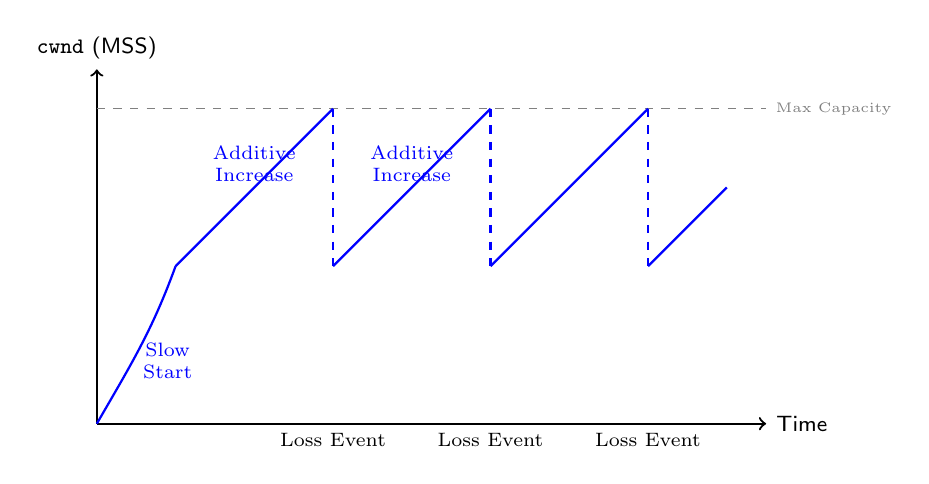
\begin{tikzpicture}
        % Axes
        \draw[->, thick] (0,0) -- (8.5,0) node[right, font=\sffamily\footnotesize] {Time};
        \draw[->, thick] (0,0) -- (0,4.5) node[above, font=\sffamily\footnotesize] {\texttt{cwnd} (MSS)};
        % Guidelines
        \draw[dashed, gray] (0,4) -- (8.5,4) node[right, font=\tiny] {Max Capacity};
        % Slow start 1
        \draw[thick, blue] (0,0) to[out=60, in=250] (1,2);
        % Additive increase 1
        \draw[thick, blue] (1,2) -- (3,4);
        % Loss event (multiplicative decrease)
        \draw[thick, blue, dashed] (3,4) -- (3,2);
        \node[below, font=\scriptsize] at (3,0) {Loss Event};
        % Additive increase 2
        \draw[thick, blue] (3,2) -- (5,4);
        % Loss event 2
        \draw[thick, blue, dashed] (5,4) -- (5,2);
        \node[below, font=\scriptsize] at (5,0) {Loss Event};
        % Additive increase 3
        \draw[thick, blue] (5,2) -- (7,4);
        % Loss event 3
        \draw[thick, blue, dashed] (7,4) -- (7,2);
        \node[below, font=\scriptsize] at (7,0) {Loss Event};
        % Resume...
        \draw[thick, blue] (7,2) -- (8,3);
        % Labels
        \node[font=\scriptsize, align=center, blue] at (0.9,0.8) {Slow\\Start};
        \node[font=\scriptsize, align=center, blue] at (2,3.3) {Additive\\Increase};
        \node[font=\scriptsize, align=center, blue] at (4,3.3) {Additive\\Increase};
    \end{tikzpicture}
    \caption{The classic TCP Sawtooth plot, illustrating Additive Increase, Multiplicative Decrease (AIMD). The congestion window grows linearly to probe available bandwidth, and drops sharply upon detecting a loss event.}
    \label{fig:tcp_sawtooth}
\end{figure}

